\documentclass[conference]{IEEEtran}

\usepackage[pdftex]{graphicx}
\usepackage[cmex10]{amsmath}
\usepackage{algorithmic}
\usepackage{caption}
\usepackage{subfig}
\usepackage{url}
\usepackage{balance}

\begin{document}
\title{What Can Stack Traces Tell us about the Use of Exceptions in Java?}

\author{\IEEEauthorblockN{Roberta Coelho\IEEEauthorrefmark{1}, Georgios Gousios\IEEEauthorrefmark{2}, Arie van Deursen\IEEEauthorrefmark{2}, Lucas Mariano\IEEEauthorrefmark{1}}
\IEEEauthorblockA{\IEEEauthorrefmark{1}Federal University of Rio Grande do Norte\\
Natal, Brazil\\
Email: \texttt{\{roberta, lucasm\}@dimap.ufrn.br}}
\IEEEauthorblockA{\IEEEauthorrefmark{2}Delft University of Technology\\
Delft, The Netherlands\\
Email: \texttt{\{gousiosg,a.vandeursen\}@tudelft.nl}}
}

\newcommand{\todo}[1]{\textbf{TODO}\footnote{\textbf{TODO:} #1}}

% make the title area
\maketitle

\begin{abstract}
Exception handling is one of the most used techniques for structuring the error recovery code of a system. Although exception handling mechanisms have been embedded in several main stream programming languages (e.g. Java, C++, C\#), studies have shown that the exception handling code is often poorly understood and the least tested parts of systems. As a consequence, the exception handling code may make the program more complex and even less reliable, leading to the so-called uncaught exceptions, one of the main causes of system crashes. Stack traces are a useful source of information to better understand such system crashes. In this work, we performed the first large scale analysis of Java stack traces and pinpoint how they can reveal bad programming practices. We mined and analyzed the stack traces embedded in all issues of Java projects available GitHub. Overall, our research set includes 16.837 projects and 58.490 stack traces. Some patterns of exception (mis)-use were consistently detected in this study, such as: most of the stack traces were related to coding errors such as null pointers; unexpected wrappings such as Errors being wrapped in checked exceptions and re-signaled; and undocumented runtime exceptions signaled by third party code.
\end{abstract}

%\IEEEpeerreviewmaketitle

\section{Introduction}

Modern applications have to cope with an increasing number of abnormal computation states that arise as a consequence of faults in the application itself (e.g., access of null references), noisy user inputs or faults in underlying midleware or hardware. The exception handling mechanism ˜\cite{goodenough1975exception} is one of the most used schemes for detecting and recovering from such exceptional conditions. Although the exception handling mechanism have been embedded in several programming languages (e.g. Java, C++, C\#) and the target of some studies [][][][], the exception handling code is often generally poorly understood and the least tested parts of systems. 

Often some languages constructions may lead the developers into believing that by just re-throwing the exceptions they can forget about the exceptional situations during the development of the "happy path". This "ignore-for-now" approach may turn the exception handling can become a kind of generalized "goto" mechanism ˜\cite{mandrioli1992advances} making the program more complex and even less reliable. This behaviour may lead to the well known uncaught exceptions problem ˜\cite{jo2004uncaught}, one of the main causes of application crashes.  

Moreover, some languages use exceptions to represent coding errors (out-of-bounds array index, division-by-zero, access to a null) in this cases exceptions are implicitly signaled by the runtime environment when such condition happens. One of such implicit exceptions (caused by data conversion from 64-bit floating point to 16-bit signed integer) was the responsible for the failure on Ariane 5's first test flight ˜\cite{lions1996ariane} - leading to the rocket self-destructing 37 seconds after launch and a loss of 500 million dollars. Besides Ariane 5, several applications crash everyday due to uncaught exceptions ˜\cite{jo2004uncaught}. In other words, the consequence of a careless exception usage may have the opposite consequence of its initial intention of improving system robustness.

In Java, when the program fails due to an uncaught exception the program automatically terminates and the system prints the stack trace which includes a detail message and the stack trace when the exception happened. A typical Java stack trace consists of an ordered list of methods that were active on the call stack before the exception has occurred. Stack traces are a useful source of information about system crashes, and is often used to support developers in debugging [ref:do stacks help]. Some works have been proposed to extract stack trace information from crash and bug reports and use stack trace information to support bug classification and clustering [][][], debugging tasks [][][] and the automated bug fixing [] task [ref], the prediction of fault proneness of classes [][]. 

However, all these works focus on the analysis of a single system at a time. In our current context, on which we have plenty access to the information available on open-source repositories like GitHub a research questions arise: What the stack traces available in these repositories can tell us about the use of exceptions in Java programs?

To answer this question, we conducted a sequential mixed-methods exploratory study [ref-mixed methods] which focused on mining the stack trace information available on all Java projects on GitHub repository, and combining this information with bytecode analysis, source-code analysis and manual inspection. 

To guide our exploratory study we firstly compiled a subset general guidelines proposed by Johua, Bertrand Myer and Rebeca (see Section X), and then using the mixed-methods described above the investigated whether we could discover whether those practices have been followed or not on the analyzed projects.A tool called ExceptionMiner, was developed in this work to mine stack trace information from Github issues and combine this information with source code and bytecode analysis.

This study was divided in two phases: in the fist phase the issues of all Java projects available on GitHub was analyzed and all available stack traces extracted using ExceptionMiner. In this first phase XXX projects were analyzed, overall containing XXXX issues, from which YYYY stack traces were extracted and used as a source of information for our analysis.

In the second phase of this study, we combined the information of the mined stack traces with sourcecode and bytecode analysis, and to do so we selected the subset of all Android applications availabe in GitHub, this subset is composed by 526 aplications (Sections X details how those aplications were selected and studied). 

We choose the Android apps available GitHub mainly because this kind of application are known for dealing with several sources of exceptions: they deal with an io-intensive infrastructure (Network, Bluetooth, camera…), and their development model involve multiple threads (ICSE arie – android specification). Moreover they are based on a single platform which allow more specific analysis of the exception behaviour.

Some negative outcomes were consistently detected through this large scale analysis of exception stack traces in the wild, such as:


\begin{itemize}
\item  A multitude of NullPointerExceptions and JVM implicitly thrown exception was found on stack traces. approximately 80\% of all stacks were related to this kind of exceptions.
\item Odd exception chains were detected: ERROR  wrappred in a checked/runtime, chacked wrapped on Runtimes and ret-thrown.
 \item  Undocumented runtime exceptions thrown by  libraries and causing crashes.
\item the use of general exceptions with no semantic associated to its type - X\% of the stack traces were caused by pure Runtime exceptions.
\item  size of stack traces whose size contained aproximately 100 method calls. Which makes the handling difficult since contextual information is lost.
\end{itemize}

During this study we implemented an stack exception mining tool which was very useful when finding and characterizing these outcomes. The contributions of this study are as follows:
\begin{itemize}
\item  It performs the first large scale analysis of Java stack traces and how they can reveal bad-practices. 
\item  It briefly presents ExceptionMiner, a tool developed to support the analysis.
\end{itemize}

The contributions of this work allow for developers of robust Java applications to familiarize with the most common reported exceptions and help developers to avoid making them; (ii) designers of  languages to consider ways of reducing the abundance of NullPointerExceptions, (iii) and tool designers to consider developing tools that enable a cross-project defect analysis. Specially in the open-source environment faults are not to be hidden in a private bug issue,faults should be share and discussed, so a developer can learn from other projects mistakes, and currently the search facilities of repositories are very limited. The ExceptionMiner tool is the fist step in this direction.

The remainder of this paper is organized as follows. Section 2 presents a background on error handling mechanisms and Java exception handling constructs and practices. Section 3 defines the hypotheses and configuration of our exploratory study, the target applications and the evaluation procedures. Section 4 reports our analysis of the empirical data collected in this study. Section 6 provides further discussions and lessons learned. Section 7 describes the related work. Finally, Section 8 presents our conclusions and directions for future work. 


%PS: OLD CONTENT OF THIS SECTION WERE REMOVED TO THE END of THIS PAPER.

\section{Background}

\subsection{Error handling in various programming languages}

Modern applications have to cope with an increasing number of abnormal computation states that arise as a consequence of faults in the application itself (e.g., access of null references), noisy user inputs or faults in underlying middleware or hardware. 

Currently, the exception handling mechanism (Goodenough, 1975), imbedded in most of the main stream programming languages, is one of the most used schemes for detecting and recovering from such exceptional conditions.


\noindent\emph{Return codes}
The main disadvantage of return codes if the fact that the programmer can just ignore the return code and let the program execute in inconsistent state.
    

\noindent\emph{Exceptions}
 Exception Handling mechanisms are embedded in many mainstream programming languages, however they differ in the way exceptions are represented and handled in each language (Garcia et al). Considering for instance the need to declare exceptions on the method signatures, several approaches can be applied. In languages such as Lore, C++, and Arche fall although all exceptions are unchecked, the developer can optionally listing exception types on method signatures. In the other hand in Modula-3, Guide, and Extended Ada the programmer must explicitly list every exception that can be signaled. Hence, all exceptions are checked exception. Java is the only language that introduced a hybrid approach. In Java, a method can throw either an instance of RuntimeException or Error, which are both unchecked and not need to be listed on the methods signature or an instance of Exception which is therefore a checked exception and must be listed in the method signature. 

\noindent\emph{Monads}
    In functional programming languages, side effects are undesirable and in
    the case of pure functional languages (e.g. Haskell) impossible. To encapsulate and 
    isolate side effects, such as exceptions, pure functional languages use monads. Monads 
    allow for composition of chains of computations that might throw recoverable exceptions 
    in a way that if an exception occurs, subsequent computations are abandoned and the 
    exception is returned as the computation result. In effect, monads wrap exceptions into
    values. An example of an exception handling monad is the \texttt{Try[T]} type in Scala. 

\subsection{Exception handling in Java}

In Java, an exception is represented according to hierarchical structure illustrated in Figure 1  (Gosling et al., 1996). According to this structure every exception is an instance of the Throwable class, and can be of three kinds: checked exceptions (extends Exception), run-time exceptions (extends RuntimeException), and errors (extends Error). 

\begin{figure}
\centering
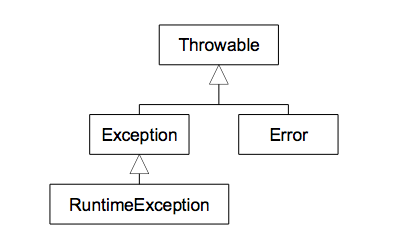
\includegraphics[scale=0.5]{exception_hierarchy.png}
\caption{Exception Hierarchy in Java}
\label{fig:Exception Hierarchy in Java.}
\end{figure}

Checked exceptions must be declared as part of the method signature that may throw it. The use of checked exceptions allows the compiler to statically check that appropriate handlers are provided within the system. The use of checked exceptions, however, is costly to maintain (Dooren and Steegmans, 2005) since every method on the call chain of a method that raises a new exception should be updated to declare this exception (on the throws clause defined on its signature) or handle it. 

On the other hand, both runtime exceptions and errors (which are also referred as unchecked exceptions) do not need to be declared on method signatures, but as a consequence there is very little that can be checked at compile time. The invalid operations in the program detected by the Java Virtual Machine are represented as runtime exceptions (e.g., NullPointerException). By convention an Error represent an unrecoverable condition which usually result from failures detected by the Java Virtual Machine, such as OutOfMemoryError - and should not be handled inside the application. 

The client of a method cannot easily know which unchecked exceptions may be thrown by the method unless he/she carefully inspects the code of the method and the methods called from it – which can become a very time consuming or infeasible task. Moreover, the developer is not warned by the compiler if an unchecked exception is not handled inside the application. For that reason the Java specification suggests that most user-defined exceptions should be checked exceptions to take advantage of compile-time checks. However, there is a long-lasting debate about the use of checked and unchecked exceptions (links to debates). There are pros and cons associated to both uses. 

\subsubsection{Exception Signaling and Handling}

In Java an exception can be signaled in one of the following circumstances [ref: java specification]:

\begin{itemize}
\item  explicitly signaled when a throw statement is executed;
\item  implicitly signaled by the JVM when the evaluation of an expression violates the normal semantics of the Java programming language.g., out-of-bounds array index, division-by-zero, access to a null reference; or 
\item implicitly signaled by the JVM due to an internal error or resource limitation (e.g., OutofMemoryError, StackOverflowError)
\end{itemize}

When an exception is signaled it causes a transfer of control from the point where the exception occurred to a point that can be specified by the programmer (exception handler). In Java it is represented by the try-catch block and is responsible for performing any recovery action necessary to bring the software system back to a normal state and, whenever this is not possible, to log the exception and abort the system in an expected safe way. 

Exception Model. In Java, as in many languages, the search for the handler to deal with a raised exception occurs along the dynamic invocation chain. This is claimed to increase the software reusability, since the invoker of an operation can handle it in a wider context (Goodenough, 1975). If no handler in the chain is found the default handler associated to the Thread or ThreadGroup is invoked (see Java Specification for more detail) which usually terminates the system and print the stack trace on the console.

\subsubsection{Exception Wrapping}
A common handling technique for Java exceptions is wrapping. With wrapping, caught exceptions
are re-thrown by the catching method in the form of a more general exception type.
Exception wrapping is useful for restring the propagation of exception types towards
upper layer methods and for hiding the exception flow (and consequently the implementation)
of components from their users. Exception wrapping is implemented by special exception
constructor methods where wrapped exceptions are passed as arguments. 

An example a multiple exception wrapping is depicted on the stack trace
 in Figure~\ref{fig:wrapping}. This stack traces was extracted from an issue of an Adroid application in Github.The bottom part of the stack trace is the \emph{root cause}, which indicates
the real reason the error was thrown (in this case, the computer run out of
memory). The top part of the stack trace indicates the location
of the exception manifestation; the stack trace is the result of no 
exception handling taking place at this part of the source code.
The intermediate blocks indicate how the exception was wrapped
while crossing API layers between the exception root location and the
exception manifestation. In all levels, the exception \emph{signaler}
method is the one that threw the exception.

\begin{figure*}
\centering
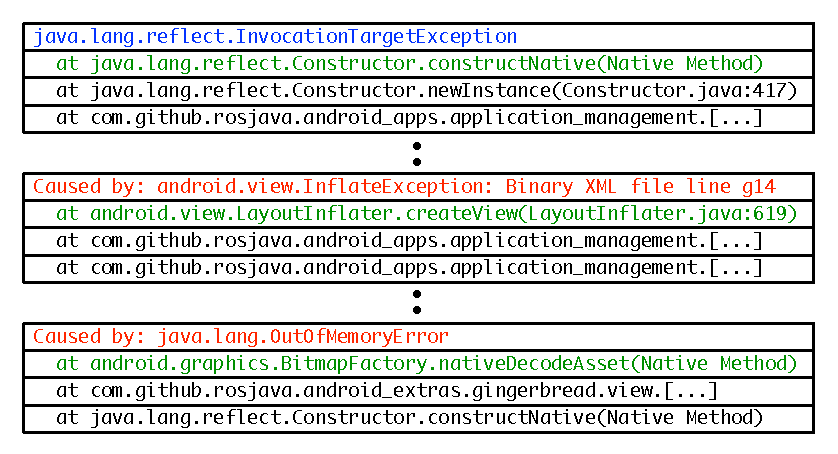
\includegraphics[scale=0.8]{wrappings}
\caption{Exception wrapping in Java stack traces}
\label{fig:wrapping}
\end{figure*}


\subsection{Exception Handling Best Practices}

Several general guidelines have been proposed on how to use exceptions in general [bertrand meyer] and in Java programs [specification-java] [Joshua] [Rebecca]. Although some of them may differ with respect to use of checked and unchecked exceptions, all them agree with the following:


\textbf{1. Exceptions representing coding errors should not be handled, then you should work to prevent them} [REBECA].  Since the implicit exceptions (out-of-bounds array index, divide-by- zero error, null pointer references) may occur in many points in the program  and recovery from them is usually difficult, they should not be handled inside the program. Otherwise a program handling such exceptions would be sprinkled with catches, and will simply be an irritation to programmers. Hence developers should use development and testing practices and tools in order to prevent them as much as possible. 

\textbf{2. Throw exceptions appropriate to the abstraction.} Higher layers should catch exceptions thrown by lower-layers and in their place throw exceptions that can be explained in terms of the higher level abstraction. To do this the developer can perform an exception translation [ref] or exception chaining. Although this practice is superior to the carelessly propagation of exceptions it should not be overused. The caller should try to prevent, handle the exception and evaluate if the exception is appropriate to the higher level.

\textbf{3. Do not repeatedly re-throw exceptions, handle exceptions as close as possible to the problem} Although exceptions don’t cost anything until they’re raised, programs that frequently raise exceptions run more slowly. Moreover, close to the place that the exception was throw the caller usually have enough contextual information to perform  corrective actions. However, when the an exception is propagated far away from the method where it was signaled (i.e. further away from the problem) it is often be difficult to take meaningful recovery actions.

\textbf{4. Errors should not be handled.} They are reserved to the JVM to indicate resource deficiencies, invariant failures and other conditions that make impossible the program to recover.

\textbf{5. Use checked exceptions for recoverable conditions.} The developer should use checked exceptions for conditions from which the caller is expected to recover. By confronting the API user with a checked exception, the API designer is telling the client to handle the exceptional condition. <<<The client can explicitly ignore the exception (swallowing, or converting it to other kind) but it is usually a bad idea.>>>

\textbf{6. Document precisely all exceptions thrown by a method} This practice is particularly important for library methods [Joshua][rebeca]. The exceptions thrown by a method are an important part of its documentation required to use the method properly. As the checked exceptions should be part of the methods signature, the method caller is aware of the checked exceptions being thrown by a method. However, it is wise to document the explicitly-signaled unchecked exceptions as carefully as the checked exceptions (in the @throws tag in Javadoc). Doing so the clients of a method will be aware of the exceptions the method can throw. If the developer fails to do follow this practice (specially for library code) it will be difficult or even impossible for the caller to make effective use of such method.


These best practices guided our exploratory study described in the next sections. Based on information extracted from stack traces and on bytecode and source-code analysis, we investigated whether some characteristics could revealed whether these practices  have been obeyed. Next section discusses the study procedure and the practices' misuses that emerged from this study.

\section{Research Design}

We used the sequential mixed-methods approach, a procedure for collecting, analyzing, and integrating both quantitative and qualitative data at some stage of the research process within a single study for the purpose of gaining a better understanding of the use of exceptions in Java programs
based mainly on the information available on exception stack traces and source code. For specific research questions, we first explore the domain quantitatively, and then highlight interesting cases by exploring 
cases qualitatively. 

Below, we present the research questions we investigate in this study and how we approach them:
\begin{description}

    \item[RQ1] What is the prevalence of stack traces on the reported issues of open-source Java programs?
    \item[RQ2] What are the most popular exceptions?
    \item[RQ3] What patterns of exception (mis)-use emerge from the stack trace analysis?

\end{description}

\textbf{RQ1} 
%What is the prevalence of exception-handling bugs on the reported issues of open-source Java programs? 
%This question should be answered in order to conduct this study. Hence if not enough exception stack traces %were reported we would not have enough information to investigate the use of best practices from stack trace information.
To assess the prevalence of exception handling bugs, we  mine and analyze statistically all issues 
from all Java projects in the Github repository.
In particular, we investigate such questions as 
what is the percentage of issues with stack traces and whether issues labeled by 
developers as defects include a stack trace.

\textbf{RQ2} To discover the most popular exceptions, we 

\textbf{RQ3} Going in depth with analyzing the extracted
stack traces requires examining individual stack trace elements and classifying
them in categories such as Java-based exceptions, library exceptions or
application exceptions. Doing the classification on all stacktraces mined from Github
is not practical as one needs to know in advance the package names exported by the application
and those exported by the libraries the application uses. 

To restrict the analysis domain, we focused our analysis on Android projects.
This decision was based on our experience
of analyzing stacktraces and was driven by the fact that most open source Android applications
make use of a rich, well-defined stack of {\sc api}s (Android) and a limited number of
shared external libraries. Moreover, Android applications are known~\todo{ref} for dealing with several sources of exceptions due to multithreaded execution and interaction with input/output resources.
%Since these applications share a common framework, and sometimes even libraries, we wanted to discover whether most of the application crashes were caused by exceptions on the application itself or exceptions signaled by the supporting framework or reused code - a study have show that there is a high degree of reuse between apps.

To answer research questions RQ2 and RQ3, we constructed a new dataset featuring
aand
analyzed it both statistically and using machine learning techniques (association rule 
mining) to 

\textbf{RQ4} complete....

\section{Data and Tools}

We begun our investigation using the dataset provided by the GHTorrent project, 
an off-line mirror of the data offered
through the Github API. The Github API data come in two forms; a streaming data flow lists events, 
such as reporting an issue, happening on repositories in real time, while a static view contains 
the current state of entities. The data is stored in unprocessed format, in a MongoDB database, 
while metadata is extracted and stored in a MySQL relational database. The GHTorrent dataset covers
a broad range of development activities on Github, including issues. The project has been collecting data since February 2012. Up to Dec 2013, when we queried it to retrieve our bootstrapping 
sample, the project had collected XXX issues from YYY Java projects.

Issues on Github are different from issues on dedicated bug tracking tools such as Bugzilla
and Jira. The most important difference is that there are no predefined fields for 
bug reporters to select from (e.g. severity and priority); Github uses instead a more open
ended tagging system. Repositories are offered a pre-defined set of labels, but repository
owners can modify them at will. An issue can have an arbitrary set of labels attached.
This meant that our analysis could not be based on labels alone 
Moreover, issue and pull requests are dual on Github; all pull requests have a corresponding 
``backing'' issue. Therefore, we needed to exclude pull request based issues from our analysis.
Finally, the Github API allows the automated generation of issues for specific repositories, 
which automated tools often use to report crashes. In some cases, this led to high number
of issues that included stack traces (e.g. ). We identified and filtered those cases out.

After obtaining the bootstrap issue sample from GHTorrent, we analyzed it in the following
ways:

\begin{itemize}

    \item We obtained the issue labels for all issues. We were especially interested in 
    issues sporting the default ``defect'' label.
    
    \item We obtained project information for each issue, separated Android projects from
    the general population of Java projects and analyzed their source code (Section~\ref{sec:android}).
    
    \item We extracted stacktraces embedded in the issue body and classified the exceptions 
    (Section~\ref{sec:datasetcons}) using the custom ExceptionMiner tool
    (Section~\ref{sec:exceptionminer}).
    
    \item We qualitatively analyzed specific stack traces (Section~\ref{sec:qualitative}).
    
\end{itemize}

\subsection{Analysis of Android projects}
\label{sec:android}

%In the second phase of this study we selected a subset of Java applications to be analyzed in more
%detail.The subset chosen was comprised by the Android apps included on GitHub (until 23 Feb 2013).
To identify Android projects, we performed a case insensitive search for the 
term \textsf{android} in the repository's names and short descriptions.
The heuristic filtered XXX repositories on which XXX issues were reported. 
We performed further cleanup, inspecting the site of every Android app analysed in this 
study to make sure that they were indeed mobile apps. X apps were removed from the
set because although having Android on its description or name they were not Android apps (e.g. 
\textsf{selendroid} -- a tool for testing android apps).

This subset consisted initially in 2.542 Android apps, from which 589 apps had at least one issue containing a stack trace. From this set 443 were analyzed in this study. \todo{How did we select those?}

\todo{What other analysis did we do? Extract packages from source code?}

\subsection{Extracting exceptions with ExceptionMiner}
\label{sec:exceptionminer}

To extract exceptions from issues, we implemented ExceptionMiner, a modular mining tool
able to connect to various repositories (such as Google Code, GHTorrent or even directly to
Bugzilla), extract issues, mine stacktraces from them and classify them in predefined categories.
The ExceptionMiner works as follows.

\noindent\emph{Stacktrace Miner} The first step in the process is mining references to exceptions and 
stack traces embedded in issues, distilling the information that composes a stack trace and storing
the results in a relational database. The extracted stack trace information  the exception signaler, the root cause, the exception wrappers. The tool is based on a combination of regular expressions in with a parser\todo{What kind of parser? Need more info...}. In contrast to existing issue parsing 
solutions such as Infozilla, the parser created in this work can extract all causes related to an 
exception on a stack, and stack traces embedded in logs files.

%\begin{tiny}
%\begin{verbatim}

%03-01 W/dalvikvm(7924): threadid=1: thread exiting with uncaught exception (group=0x40adf210)
%03-01 15:55:01.609 (7924): FATAL EXCEPTION: main
%03-01  (7924): java.lang.RuntimeException: ...
%E/AndroidRuntime( 7924):  at android....performLaunchActivity(ActivityThread.java:1967)
%03-01 15:55:01.609 (7924):  at android....handleLaunchActivity(ActivityThread.java:1992)
%03-01 15:55:01.609:  at android.app.ActivityThread.access\$600(ActivityThread.java:127)
%E/AndroidRuntime( 7924):  at android....handleMessage(ActivityThread.java:1158)
%\end{verbatim}
%\end{tiny}

\noindent\emph{Exception Classifier} The next step in the ExceptionMiner process is classifying exceptions as either checked exceptions, runtime exceptions or an errors. The exception classifier
is based on bytecode analysis (based on ASM [REF]) that walks up the type hierarchy of a Java exception until it reaches a base exception type. 

\noindent\emph{Exception Singaler Classifier} The final step is finding and classifying 
information about exception signalers. ExceptionMiner is initialized with an arbitrary 
set of packages for each classification category and pattern matches the signaler name
to classify it to one of the categories. 

\subsection{Dataset Construction}
\label{sec:datasetcons}

We applied the ExceptionMiner tool on the whole set of issues in our bootstraping sample
and then independently on the set of issues from Android projects. 
In the first case the exception classifier was initialized with all the exceptions defined on
the Java SDK version 7, while the signaler classifier was configured with Java's package
names.
In addition to the above, for the Android dataset analysis, the exception classifier
was initialized with the exceptions of the Android 
platform (level X), and all the exceptions of the 443 Android projects selected for this study.
The signaler classifier was initialized with information
about all packages that compose Java Environment, all packages composing all versions of Android Platform (Operating System and Framework), all packages that compose the core libraries reused by the Android API and all packages of 443 out of the 529 mobile apps hosted in Github which defined at least one issue that contained a stack trace \todo{this list of all packages can be found at [site].}.
What we could not classify in one of the above categories was automatically labeled as a library.



\section{Study Operation and Results}
This section presents the results for each of the study phases, providing both a quantitative and qualitative analysis of the outcomes. Firstly (Section X) we present the results of inspecting all Stack Traces  of Java Programs considered in this study. The following section focuses....

%\subsection{Phase 1: Analyzing Pure Stack Trace Information of Java Programs}

\subsection{RQ1: What is the prevalence of exception-handling bugs on the reported issues of open-source Java programs?}

% latex table generated in R 2.15.3 by xtable 1.7-1 package
% Mon Apr 28 15:44:10 2014
\begin{table*}[ht]
\centering
\begin{tabular}{rp{27em}rrrrc}
  \hline
Feature & Description & quant\_5 & mean & median & quant\_95 & histogram \\ 
  \hline
   \multicolumn{2}{l}{\bfseries{Java}}  \\
all & All issues recorded for the project. & 1.00 & 23.37 & 3.00 & 80.00 & 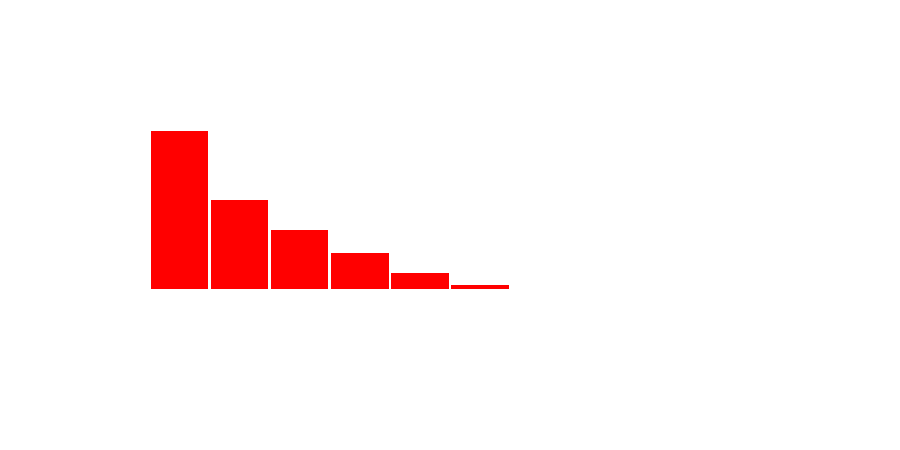
\includegraphics[scale = 0.1, clip = true, trim= 50px 60px 50px 60px]{hist-31b77719e3773ad7ac2073785de62a5f.pdf} \\ 
  with\_exception & All issues featuring an exception. & 0.00 & 3.21 & 0.00 & 6.00 & 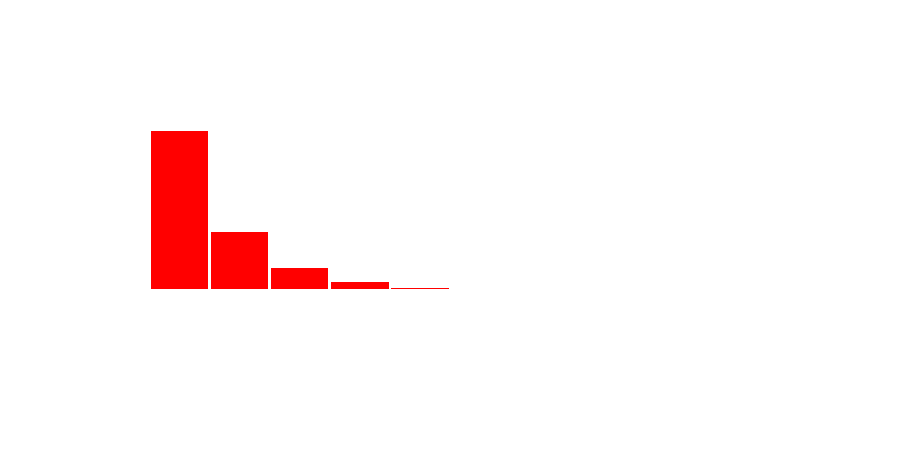
\includegraphics[scale = 0.1, clip = true, trim= 50px 60px 50px 60px]{hist-0c1305fc40f695dbdd1f4696db24f147.pdf} \\ 
  with\_stack & All issues featuring a stack trace. & 0.00 & 2.67 & 0.00 & 4.00 & 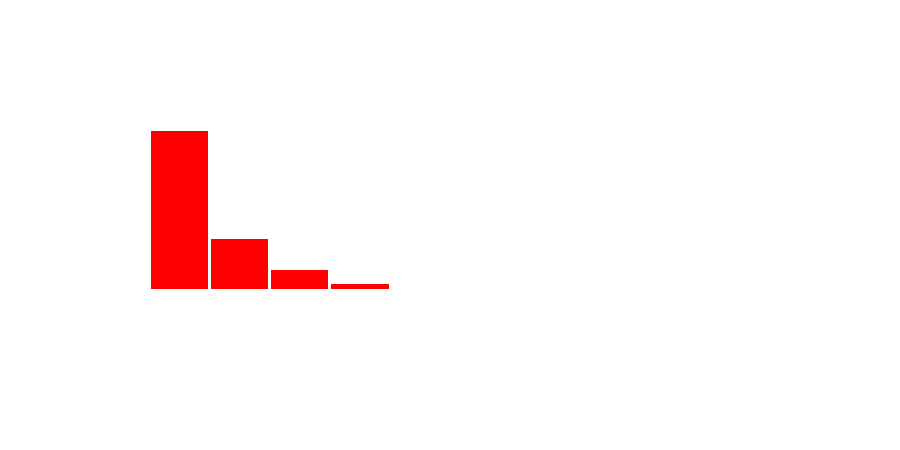
\includegraphics[scale = 0.1, clip = true, trim= 50px 60px 50px 60px]{hist-896524802e915aa3f01ef1ecd2489e7e.pdf} \\ 
  defect\_issues & All issues labeled as defect. & 0.00 & 5.51 & 0.00 & 12.00 & 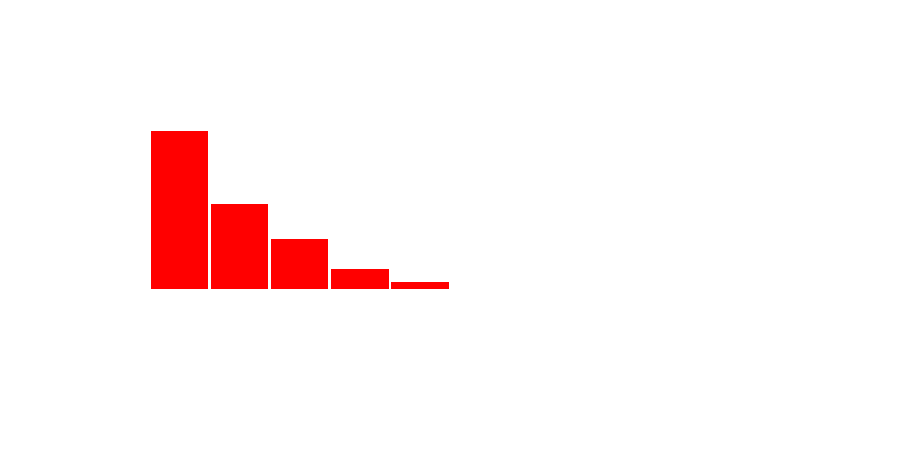
\includegraphics[scale = 0.1, clip = true, trim= 50px 60px 50px 60px]{hist-5d0ab95cd3e300c21b0a40d6bec58e4c.pdf} \\ 
  defect\_with\_exception & All issues labeled labeled as defect and including an exception. & 0.00 & 1.82 & 0.00 & 1.00 & 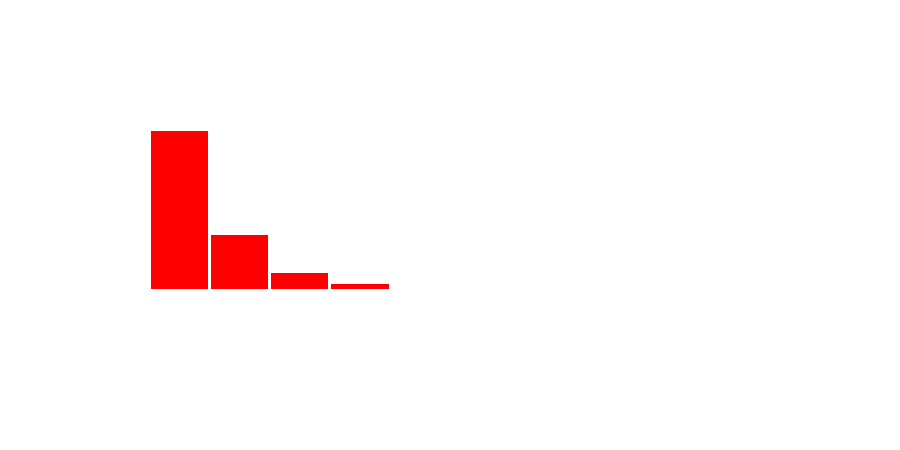
\includegraphics[scale = 0.1, clip = true, trim= 50px 60px 50px 60px]{hist-502028d1a7e2e77414e2f9f63e0bcd50.pdf} \\ 
  defect\_with\_stack & All issues labeled labeled as defect and including a stacktrace & 0.00 & 1.73 & 0.00 & 1.00 & 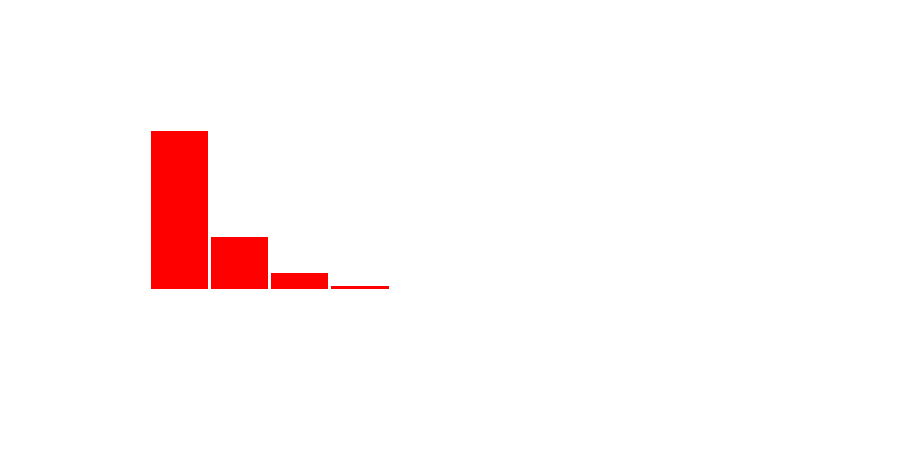
\includegraphics[scale = 0.1, clip = true, trim= 50px 60px 50px 60px]{hist-dab0764147debd99066c84814d46d50e.pdf} \\ 
   \hline
   \multicolumn{2}{l}{\bfseries{Android}}\\
   all & All issues recorded for the project. & 2.00 & 67.70 & 20.00 & 248.00 & 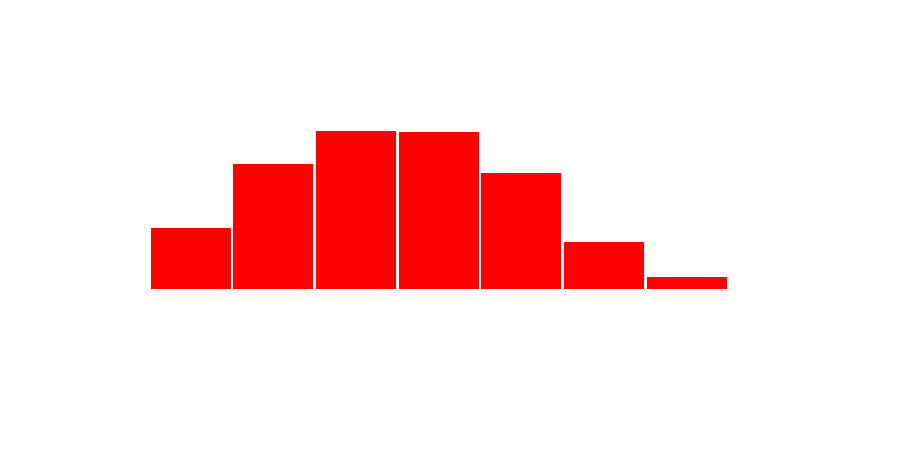
\includegraphics[scale = 0.1, clip = true, trim= 50px 60px 50px 60px]{hist-5d4a87daa44c63097df9bb1f3506d541.pdf} \\ 
  with\_exception & All issues featuring an exception. & 1.00 & 8.16 & 2.00 & 34.00 & 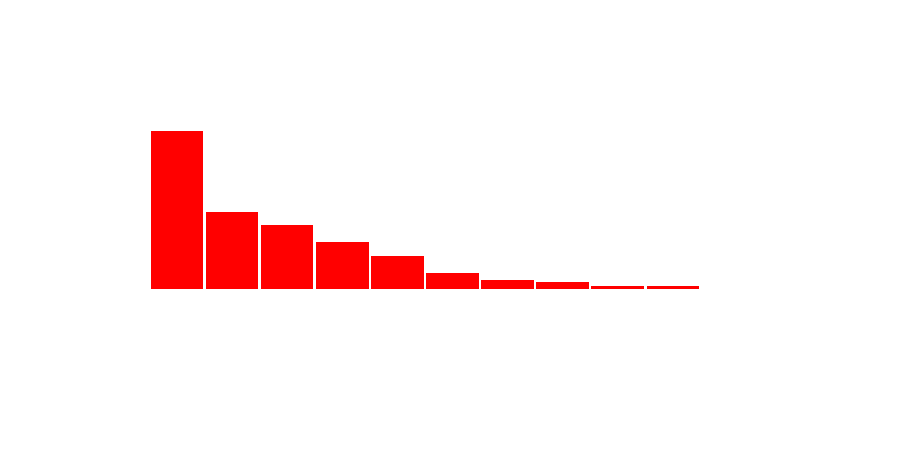
\includegraphics[scale = 0.1, clip = true, trim= 50px 60px 50px 60px]{hist-bf73235d0503f937ef6f36c28cf1ba0d.pdf} \\ 
  with\_stack & All issues featuring a stack trace. & 1.00 & 6.44 & 2.00 & 27.00 & 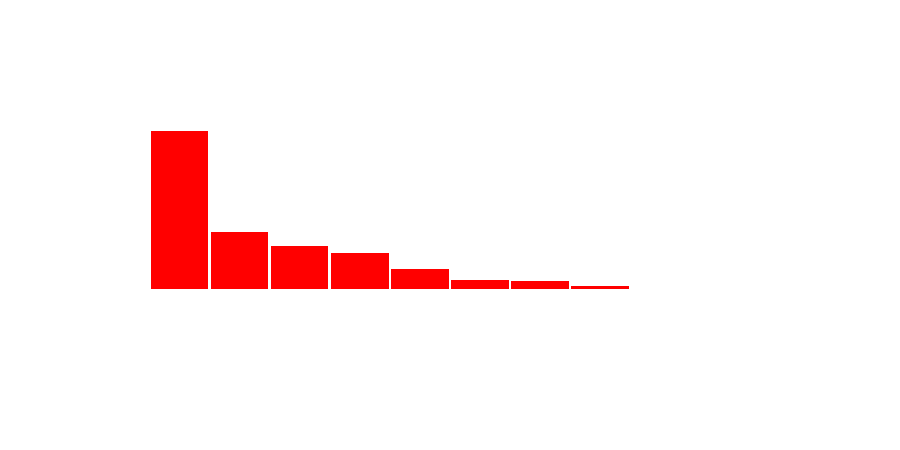
\includegraphics[scale = 0.1, clip = true, trim= 50px 60px 50px 60px]{hist-528cb6be67074e6e2c22d11245920e13.pdf} \\ 
  defect\_issues & All issues labeled as defect. & 0.00 & 13.28 & 1.00 & 52.00 & 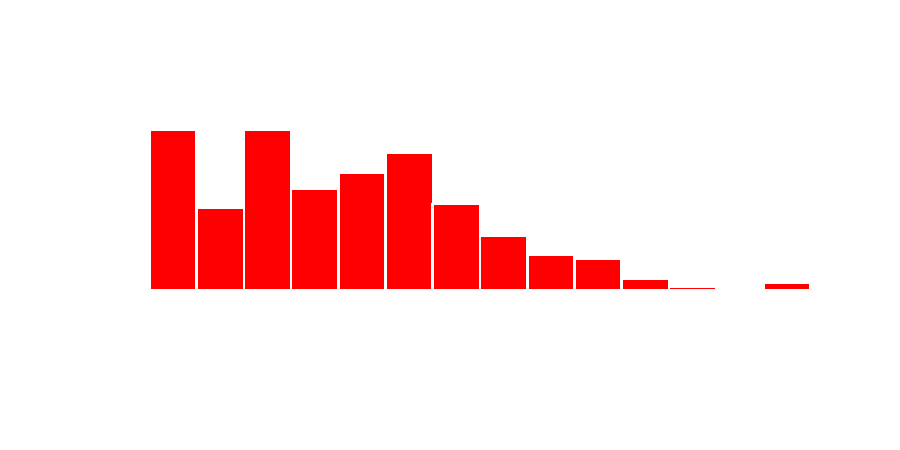
\includegraphics[scale = 0.1, clip = true, trim= 50px 60px 50px 60px]{hist-eb1797e86ef23b2a07907e5ccbeff7b9.pdf} \\ 
  defect\_with\_exception & All issues labeled labeled as defect and including an exception. & 0.00 & 3.25 & 0.00 & 13.00 & 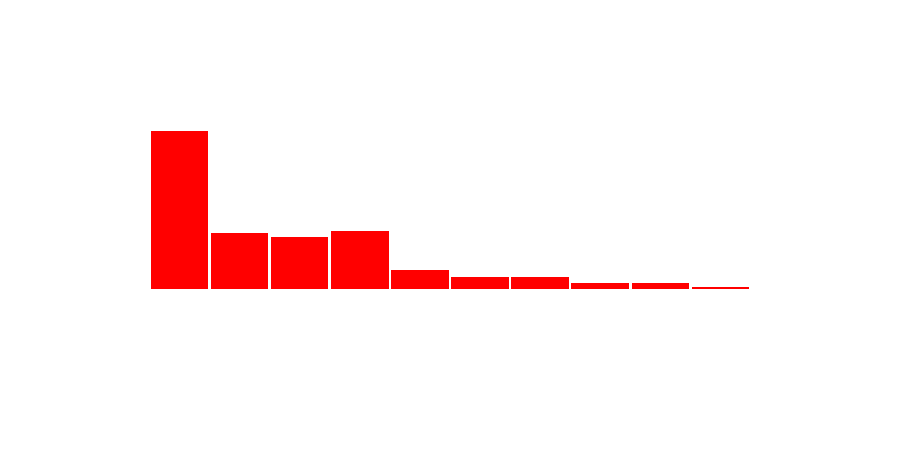
\includegraphics[scale = 0.1, clip = true, trim= 50px 60px 50px 60px]{hist-f1a879616aa3e0995db35c6c02bc8520.pdf} \\ 
  defect\_with\_stack & All issues labeled labeled as defect and including a stacktrace & 0.00 & 2.92 & 0.00 & 10.00 & 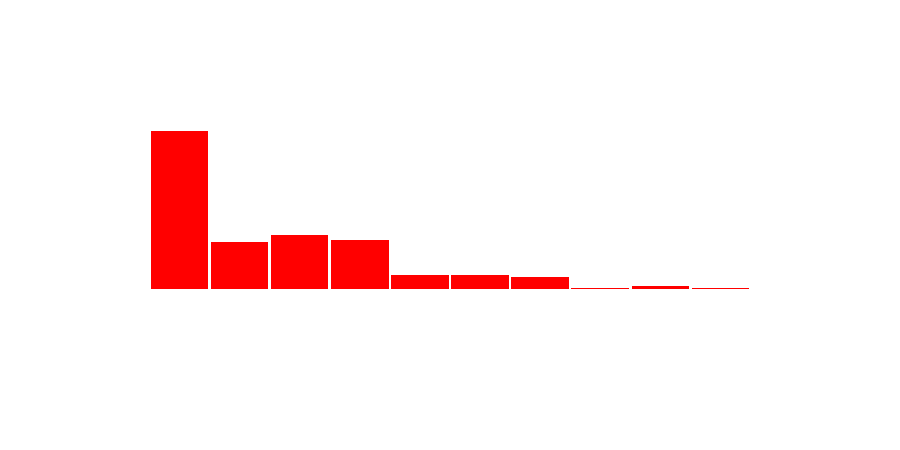
\includegraphics[scale = 0.1, clip = true, trim= 50px 60px 50px 60px]{hist-49dbfa02c366cab8b489f33014de587d.pdf} \\
 \hline
 \end{tabular}
\caption{Descriptive statistics for the analyzed issue dataset. Historgrams are in log scale.} 
\label{tab:stacktrace-stats}
\end{table*}


\begin{table}
\centering
\begin{tabular}{p{1em}lrr}
\hline
 \bfseries{Metric} & & \bfseries{Java} & \bfseries{Android}  \\
\hline
 \multicolumn{2}{l}{\bfseries{Repositories}} & 16,837 & 2,542\\
    & incl. exception on 1+ issues & 4,777 (28,37\%) & 729 (28,68\%)\\
    & incl. stack trace on 1+ issue & 3,759 (22,33\%) & 589 (23,17\%)\\
    & incl. exception on 1+ issue labeled as defect & 2,020 (41,44\%) &  329 (47\%)\\
    & incl. stacktrace on 1+ issue labeled as defect  & 1,699 (34,86\%) & 293 (41,86\%)\\
 \multicolumn{2}{l}{\bfseries{Issues}} & 393,552 & 50,342\\
    & incl. exceptions & 54,113 (13,75\%) & 4,947 (9,83\%) \\
    & incl. stacktraces & 44,886 (11,41\%) & 3,693 (7,34\%) \\
    & labeled as defect & 55,228 & 8,751 \\
    & labeled as defect and incl. exception & 6,741 (12,21\%) & 1,719 (19,64\%) \\
    & labeled as defect and incl. stacktrace &  5,196 (9,41\%) & 1,508 (17,23\%)\\
\multicolumn{2}{l}{\bfseries{Exception Stack Traces}} &  & \\
    & on issues  & 58,490  & 4,714  \\
    & on issues labled as defect & 6,529 & 1,813 \\
 
\hline
\end{tabular}
\caption{Quantitative overview of the analyzed dataset}
\label{tab:overview}
\end{table}

%\begin{figure*}
%        \centering
%        \subfloat[Java\label{fig:stacks-java}]{
%                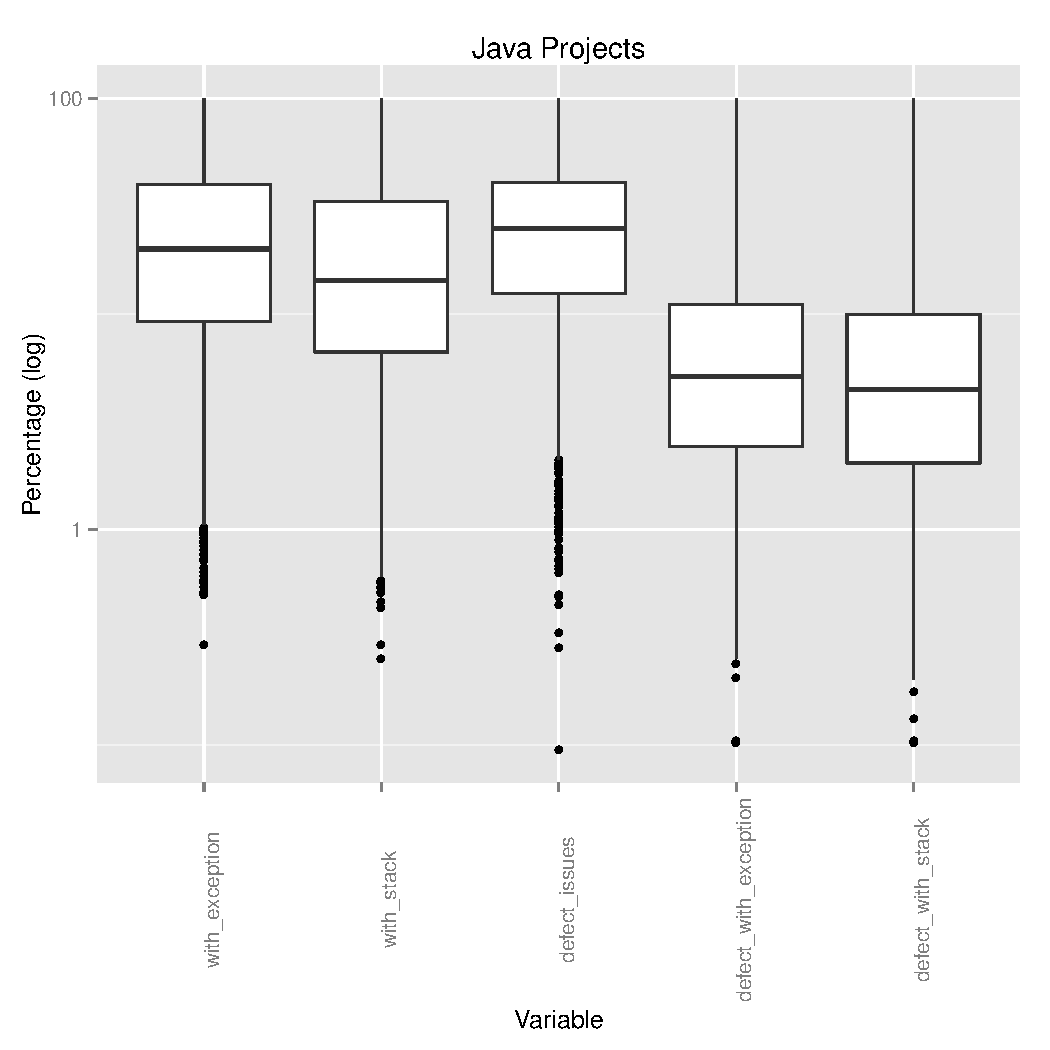
\includegraphics[scale=0.4]{java-stacks}
%        }
%        \subfloat[Android\label{fig:stacks-android}]{
%            \includegraphics[scale=0.4]{android-stacks}
%        }
%        \caption{Distribution of issues containing stack traces as 
%        percentage of total issues in Java (a) and Android (b) projects}
%        \label{fig:stacktraces}
%\end{figure*}

The use of the Github issue tracker in repositories hosted on Github is optional
and not widespread. 
As of March 2014, from the 332,864 non-fork Java repositories registered in the 
GHTorrent dataset, only 44,323 have received an issue report in their lifetime
while from those only 16,837 are being watched by external users.
To ensure that our work targets projects that are openly used by 
users other than their developers, we focused our analysis on just those
projects. Using the heuristics presented in Section~\ref{sec:postprocessing}, 
we identified 2,542 repositories featuring Android projects.
Moreover, a typical issue on Github sports a collection of labels. Labels
can be user specified, but it is common for repositories to use the default set
provided by the Github issue tracker. Consequently, we used the ``defect'' label
as a marker for issues that might contain stack traces.
Table I and Table~\ref{tab:overview} presents two views of the extracted dataset,
namely grouped by repository and grouped by issue.

At the repository level, issues that include exceptions and stack traces
are fairly common: 28\% and 22\% of the repositories include at least
one issue with either of the two. At the individual issue level, 
11\% and 13\% contain exceptions. The numbers are similar if we
isolate Android projects from the general population. This means
that focusing on Android, as we do in the next section, does not affect the 
generalizability of results at least at the sample representativeness  
level. The ``defect'' label adds context to the analyzed issues in the
Android case, as almost 20\% of the issues marked as defects include
a stack trace. This is not true for the general case however. We therefore
did not use this label for further filtering.

The results in Table~\ref{tab:overview} are cumulative; however, the numbers
are not the same among all projects. Figure~\ref{fig:stacktraces} 
presents boxplots of the range of values of the variables described in  
Table~\ref{tab:overview} across all projects in out dataset. 
There we can see that indeed there is significant variation among projects,
while the outliers lay at the bottom end of the spectrum, which means that for
some projects, we can find very limited number of stacktraces in their 
issue reports. Both Java and Android projects feature similar variation,
which again supports our Android focused analysis later on.

\noindent \fbox{ \begin{minipage}{0.96\columnwidth} \emph{
RQ1: 28\% of Java repositories on Github have issues that include
stacktraces; 11\% of all the issues in those repositories include
stacktraces. The Android issue sample is more homogenized.
}
\end{minipage}}


% \begin{itemize}

%     \item What are the most ``popular'' exceptions and what they can tell us?
    
%     \item Which elements are triggering most of the exceptions and what they 
%     can tell us about the exception structure?

%     \item What is the role of libraries and the underlying platform on crashes?

%     \item What is the role of the application itself on crashes?
% \end{itemize}

% \subsection{The rules of using checked and unchecked exceptions are being obeyed in mobile environment?}


\subsection{RQ2: What are the most popular exceptions?}

What are the main causes of exceptions on reported issues? To answer this question we mined the following information of every extracted stack trace: the top level exception being signaled, its signaler (the first method signature frame after the exception), the root exception (the exception which initiated the stack trace, defined on the bottom of the stack), and the root signaler. The intermediate elements that compose a stack trace as shown in Figure 1 (i.e., the intermediate causes and its execution stacks) were not be considered in the analysis.

Table~\ref{tab:toptenpopular} illustrates the top 10 most signaled exceptions - which represents X\% of the analyzed set. The table illustrates  (i) the number of times each exception appeared as the root cause of a stack trace (\#occurrences), (ii) the number of distinct projects reporting such causes on stack traces, and (iii) the exception popularity. The exception popularity metric was defined in this work as follows: (popularity = number of projects mentioning the exception in at least one stack/all projects that contain at least one stack).

\begin{table}
\begin{tabular}{lrr}
    \hline
    \bfseries{Exception} & \bfseries{Num Occurrencies} & \bfseries{Num Projects} \\
    \hline
      java.lang.NullPointerException &	13180 &	1671 \\
      java.lang.IllegalArgumentException &	1765 &	670 \\
      java.lang.ClassNotFoundException &	1166 &	506 \\
      java.lang.IllegalStateException &	11408 &	431 \\
      java.lang.RuntimeException &	1158 &	411 \\
      java.lang.ClassCastException &	886 &	408 \\
      java.lang.NoSuchMethodError &	838 &	370 \\
      java.lang.ArrayIndexOutOfBoundsException &	807 &	334 \\
      java.io.IOException &	646 &	316 \\
      java.lang.NoClassDefFoundError &	557 &	299  \\
      java.lang.OutOfMemoryError &	597 &	235 \\
    \hline
  \end{tabular}
\caption{Top 10 most popular exceptions on issues}
\label{tab:toptenpopular}
\end{table}

\textbf{TO DISCUSS: We can include a longer list order by the percentage of ocurrences until we reach 80\% of the 
exceptions. It means top 20 and includes some exceptions signaled by android.}

\textbf{TO DISCUSS: We can also include the top 10 excepption packages...}

We could observe that the NullPointerException was the one with the higher number of occurrences (22,5\% of all stacks were caused by NullPointerExceptions) and the one which had the highest popularity. We could also observe that most of the exceptions in the TOP 10 list (except java.lang.IllegalArgumentException, java.io.IOException and java.lang.RuntimeException) are exceptions implicitly signaled by Java Virtual Machine when an expression violates the normal semantics of the Java programming language (e.g. ArrayIndexOutOfBounds) or due to an internal error or resource limitation (OutOfMemoryError). 

The high prevalence of NullPointerExceptions, and the other implicitly-thrown exceptions  is aligned with the findings other works [Sunghun et al.][Gordon fraser and][Jcrasher].[Android-predict]. For instance, Sunghun et al. showed that in Eclipse bug report system 38\% the bugs related to exception handling were caused by NullPointerException; other works on robustness testing [JCrasher, Evol;suite, Amiya] showed that most of the automatically detected bugs were due to NullPointerExceptions and implicitly-signaled of Java environment (as the ones found in this study).


To better understand the main causes of such exceptions we evaluated specification and semantics of the top 100 root exceptions reported on stack-issues, and classified them according to the the categories presented in Table~\ref{tophundrend}.

\begin{table}
  \centering
  \begin{tabular}{lrr}
    \hline
    \bfseries{Category} & \bfseries{Occurrences} & \bfseries{Num Projects} \\
    \hline
      java.lang and util programming logic & 40857	(80,59\%) &	4874 (52,62\%)
      \\
      Resources(NET, IO, FILE) & 4445 (8,77\%) &	2121 (22,90\%)\\
      Security & 351 (0,69\%) &	132	(1,43\%) \\
      Concurrency	& 633 (1,25\%) &	290	(3,13\%) \\
      Backward compatibility & 2112 (4,17\%) &	948	(10,23\%) \\
      Reflection &	299	(0,59\%) &	195	(2,11\%) \\
      Specific (GUI,FRAMEWORK) &	600	(1,18\%) &	153	(1,65\%)\\
      General (Error, Exception, Runtime)	& 1401 (2,76\%) & 550	(32,91\%)\\
    \hline
  \end{tabular}
  \caption{Top 100 exceptions were studied and classified according to its semantics in the following categories.}
  \label{tab:tophundrend}

\end{table}

As we can see from Table 4, the that programming errors are responsible for more than 80\% of the issues reporting a stack trace. Such high prevalence points to the fact that developers may not have been using tools [ref: tools to prevent null...] and practices to prevent from such mistakes or that it may be difficult to do so (specialy in the case of NullPointerExceptions). 

\section{What kinds of exception (mis)-use emerge from stack trace analysis? }

To answer this question we analyzed information extracted from stack traces in combination with source code and bytecode analysis. As mentioned before (Section X) in the second phase of this exploratory study we focused on 443 Android projects. We downloaded the latest master version of each Android app, extracted its packages, and the user defined exceptions and run a bytecode analysis tool to classify exception mentioned on at least one stack trace as Runtime, Checked, or Error. 

Since we downloaded the latest version of each app, when an exception had been removed from the latest version we used the search facilities of Github to locate the exception code. The ones that could not be found, even through this search interface, were remained as UNDEFINED and represented X\% of the exceptions being analyzed. Besides downloading and analyzing the code of every user defined exception, we also download and analyzed the exception defined on reused libraries mentioned on stacks and every exception defined on Java Environment and Android development kit and android platform. After the massive mining effort we could come up with the findings presented in Table~\ref{typeroottab} and Figure~\ref{typeroot}.

Next sections details what patterns of exception (mis)-use emerge from this analysis.

\subsection{A multitude of NullPointerExceptions and other implicitly signaled exceptions signaled by Third Party}

After extracting every package related to each exception signaler (see Section III-B) we could classify every stack trace based on its root signaler as presented in Table~\ref{signalers}.

\begin{table}
  \centering
  \begin{tabular}{rp{22em}}
    \hline
    \bfseries{Type of signaler} & \bfseries{Description} \\
    \hline
    \bfseries{android} &	When the exception signaler is a method defined in Android Platform.\\
    \bfseries{app} &	If the exception signaler was defined inside an application class.\\
    \bfseries{libcore} &	If the application was signaled by one of the libraries reused by Android Platform. The complete list of core libraries can be found here\\
    \bfseries{lib} &	If the exceptions was not defined by any of the elements above.\\
    \bfseries{java} &	If the application signaler and all the methods that composes the exception are defined on java. packages\\
    \hline
  \end{tabular}
  \caption{Sources of exceptions in Android}
  \label{tab:signalers}
\end{table}

For each exception we could discover: the number of times it occurred on stacks, the number of distinct projects such stacks were defined (and consequently its popularity) and the of times it was signaled by different signaler types. We could calculate the popularity of each root cause, considering the number of distinct projects they were found and the whole set of projects analyzed with at least one stack trace (443). Table ~\ref{overviewandroid} and Figuere~\ref{androidsignaler} presents the mined data.

\begin{table*}
  \centering
  \begin{tabular}{rcccccccc}
    \hline
    \bfseries{Root exception} & \bfseries{Projects} & \bfseries{Popularity} & \bfseries{Occurences}	& \texttt{android} & \texttt{libcore} & \texttt{app} & \texttt{lib} & \texttt{java} \\
    \hline
    java.lang.NullPointerException	& 238	& 53,72\%	& 1244 (X\%)	& 461	& 18	& 506	& 257	& 2 \\
    java.lang.IllegalArgumentException & 100 & 22,57\% & 275  (X\%) & 166 & 3 & 52 & 54 & 0 \\
    java.lang.RuntimeException & 96 & 21,67\% & 251 (X\%) & 182 & 0 & 46 & 23 & 0 \\
    java.lang.IllegalStateException & 93 & 20,99\% & 250 (X\%) & 164 & 10 & 30 & 45 & 1 \\
    java.lang.OutOfMemoryError & 50 & 11,29\% & 166 (X\%) & 117 & 13 & 8 & 23 & 5 \\
    java.lang.IndexOutOfBoundsException & 48 & 10,84\% & 135 (X\%) & 51 & 0 & 63 & 20 & 1 \\ 
    java.lang.NumberFormatException & 36 & 8,13\% & 114 (X\%) & 17 & 4 & 81 & 8 & 4 \\
    java.lang.ClassCastException & 44 & 9,93\% & 113 (X\%) & 50 & 0 & 38 & 25 & 0 \\
    java.lang.NoClassDefFoundError & 40 & 9,03\% & 74 (X\%) & 9 & 0 & 27 & 37 & 1\\
    java.io.IOException & 32 & 7,22\% & 70 (X\%) & 14 & 7 & 28 & 20 & 1\\
    android.database.sqlite.SQLiteException & 28 & 6,32\% & 63 (X\%) & 63 & 0 & 0 & 0 & 0\\
    java.lang.SecurityException & 21 & 4,74\% & 63 (X\%) & 60 & 0 & 0 & 3 & 0\\
    java.lang.ClassNotFoundException & 40 & 9,03\% & 62 (X\%) & 46 & 0 & 3 & 13 & 0\\
    java.lang.ArrayIndexOutOfBoundsException & 30 & 6,77\% & 60 (X\%) & 15 & 0 & 27 & 18 & 0\\
    java.lang.NoSuchMethodError & 38 & 8,58\% & 58 (X\%) & 11 & 0 & 31 & 16 &
    0\\
    java.util.ConcurrentModificationException & 17 & 3,84\% & 54 (X\%) & 4 & 0 & 35 & 15 & 0\\
    \hline
  \end{tabular}
\caption{Root Exceptions occurrences and popularity.}
\label{tab:overviewandroid}
\end{table*}

\begin{figure}
\centering
\includegraphics[width=\hsize]{pic4.png}
\caption{Exception distribution per signaler type}
\label{fig:androidsignaler}
\end{figure}

We could also observe that the NullPointerException is still the exception with higher number of occurrences. The NullPoiterExceptions are mainly signaled inside Android platform and inside application code. Although we also find NullPointerExceptions being signaled from third-party libraries. Specially when dealing the reusable code, the methods should make explicit the contrat of use, and usually instead of rethrowing a NullPointerException, the resused method should rethrow an IllegalArgumentException, and document it on its signature. The same applies for android, since adroid platform offers a set of methods that will be reused by apps. Making such exception handling behaviour explicit, many of those bugs could be prevented/avoided.

Another observation was the high prevalence of RuntimeExceptions being thrown by the Android platform. We could observe that most of the RuntimeExceptions were signaled by Android Platform (182 out of 251). Such exception is to general that we can know what caused the exception if we read the exception message on the stack trace. Inspecting the code of Android Platform we could observe that is is almost an exception handling policy to convert different kinds of application (both checked and unchecked) in a RuntimeException. The code snipet below was extracted from Android platform level X and illustrate this:

If we focus on the top-level exceptions only, in other words, the ones wrapping the root exceptions. We can observe that the number of occurrences and the popularity of RuntimeException considerably increases when compared to the number of RuntimeExceptions being signaled as a root exception. 

TO DECIDE: Do we need to include the same Table showing Top Level Exceptions occurrences and popularity???

Manually inspecting the code on which RuntimeExceptions  were signaled as root exceptions and also as top level exception we could observe that RuntimeExceptions are strongly used by Android to wrap several kinds of exceptions. This wrapping behaviour may happen for 2 main reasons:  to by-pass Java checked exception rules, or simply because there is no reasonable way of handling the exception, and hence regardless the kind of exception being signaled, there is only one kind of handling (present an error message and abort/restart the application). This  shades a light in the need of robustness and fault tolerant solutions to deal with exceptional situations other than just presenting a error window.

\textbf{We could observe in this study that the NullPointerException and other other implicitly signaled exceptions represented aproximatey 80\% of all exceptions reported on issues in both Java and Android subset.
For such exceptions - which represent programming bugs or resource limitations - there is usually no proper handling besides presenting an error message to the user and restarting the application - only high fault tolerant systems need to provide solutions to handle them [REF: Java Specification]. Hence such exceptions should be prevented through the adoption of tools and techniques instead of handled in runtime. Some research works have proposed NullPointer analysis tools to statically find such potential null references [ref-ref-daniele], or testing tools targeting this kind of bug or even program transformation approaches to prevent such null references [ref]. However, we can observe that in practice such strategies are not been used. Maybe because the developers are not aware of the extent of the problem – as this study revealed that most of the crash reports were related to NullPointerException. This finding points to a broader discussion on the use of exception and how difficult is to prevent NullPointerExceptions in Java detailed in Section X.}

\subsection{Uncaught Checked Exceptions}
\begin{table}
\centering
\includegraphics[width=\hsize]{table7.png}
\caption{Types of Root Exceptions.}
\label{fig:typeroottab}
\end{table}

\begin{figure}
\centering
\includegraphics[width=\hsize]{pic2.png}
\caption{Distribution of Checked and Unchedked...}
\label{fig:typeroot}
\end{figure}

We could observe for instance that most of the exceptions reported were RUNTIME xxxx, and most of such exceptions were signaled by ANDROID environment and the application itself. <complete> 

If we consider the top level exceptions can see from Table ~\ref{wrappingtop}. 

\begin{table}
\centering
\includegraphics[width=\hsize]{table8.png}
\caption{Types of Top Level Exceptions.}
\label{fig:typetop}
\end{table}

\subsubsection{Undocumented Runtime Exceptions signaled by Third-Party code}
We could observe that most of the exceptions signaled by Android libcore where mostly checked exceptions, so they define a precise exception behaviour to its clients. However, most of the exceptions signaled by other third-party libraries reused by apps signaled mostly Runtime exceptions. 

We did a sampling study on the signaler which explicitly signaled Runtime exceptions. Our goal was to observe the whether the runtime exceptions were as carefully documented as the checked exceptions signaled by the methods. In our analysis none of the inspected methods included a documentation to it on Javadoc annotation or in the throws declaration. The lack of care developers have while documenting Runtime exceptions is aligned with the results of other studies such as the one from Cabral and Marcques who observed that ..... [ref: Cabral at al]

The undocumented RuntimeExceptions is indeed a serious problem once it makes very difficult or even impossible for the  client method to protect against such undocumented runtime exceptions.

\textbf{When libraries are used, the developer does not have access to their source code and thus needs to rely on the library documentation about the runtime exceptions that should be thrown – which, more often than not, are neither complete nor precise (Thomas, 2002; Sacramento et al., 2006). 
As a consequence, unhandled unchecked exceptions can be seen as one of the major sources of bugs in current Java systems (Jo et al., 2004). }

\subsubsection{Odd Wrappings}
The difference on the types of top level to root exceptions stimulated us to inspect the kinds of wrappings that happened on stacks based on the kinds of exceptions being wrapped.  Table ~\ref{wrappingandroid} presents the wrappings found in this study. As we can see this analysis revealed unexpected wrappings such as CHECKED wrapping an  ERROR; ERROR wrapping a CHECKED exceptop; RUNTIME - ERROR; ERROR wrapping RUNTIME.


\begin{figure}
\centering
\includegraphics[width=\hsize]{table9.png}
\caption{Kinds of wrappings found on the stacks of 443 ANDROID projects found on Github}
\label{fig:wrappingandroid}
\end{figure}

Java is the only language that provides a hybrid exception handling mechanism which offers different types to represent different exception behaviors. According to Java specification Errors represent XXXX and for that reason should not be handled most of the application since they represent. Checked exceptions represent situation from which a recovering is possible. Runtime exceptions represent.... Although the use of Runtime and Checked exceptions are not a consensus the meaning of each type of exception should be .... 
Since there is no way of enforcing such conventions during program development,  we could observe that, in practice, in some situations (illustrated by the Odd-Wrappings) these three types of exceptions were used interchangeably. This interchangeability makes the behaviour of the exception handling code more complex and less reliable. For instance, considering a situation were an OutOfMemoryError (a situation that should not be handled) was wrapped in a checked exception (a situation that must he handled), in this case this wrapping is telling to the caller that it should handle

One may think that these strange wrappings may be a characteristic of this analyzed Android apps. However, since some of the wrapping were related to static blocks and reflection library, and both also happen in other Java projects, we can foresee that these wrappings also happens. But to get a brief  notion on the size of this scenarios we re-run the analysis for the whole java set – reusing the same exception classification of the initial analysis. Since this set contains XX distinct exceptions from which XXX were previously classified in the previous study, we could observe more instances of UNDEFINED exceptions. We could actually see that these strange wrappings also happened in Java projects as illustrated in Table ~\ref{wrappingjava}. 
\begin{table}
\centering
\includegraphics[width=\hsize]{table10.png}
\caption{Kinds of wrappings found on the stacks on Java projects}
\label{fig:wrappingjava}
\end{table}

TO DISCUSS: We could also not include this table anymore, once Android was chosen lets stick to it until the end.
TO INCLUDE Table X: Kinds of wrappings found on the stacks of XXX Java projects found on github.

\subsubsection{Long Stack Traces}
One of the general guidelines on exception handling says that the developer should not repeatedly re-throw exceptions, (s)he should handle exceptions as close as possible to the problem. To investigate this practice we analyzed the number of wrappings on each stack trace and also the number of frames composing them. The resuls of this analysis are presented in Table X.


\begin{table}
\centering
\includegraphics[scale=0.5]{tablesize.png}
\caption{Kinds of wrappings found on the stacks on Java projects}
\label{fig:wrappingjava}
\end{table}

Exception wrappings happened in approximately X\% of all stack traces. We could observe that in many cases (xxx) the number of wrappings was higher than XX.

Moreover, another interesting observation is related to the size of the stacks (i.e. the number of frames composing them) which sometimes exceeded 100 frames (in XXX stack traces) the corresponding execution trace was caused by one of the two reasons:  recursive calls - ;exceptions signaled by a method defined deep down in a reused framework. Every time a third party code is reused together with the desired functionality comes exceptions (checked or runtime) related to it. We could observe that XX\% of stack traces whose size was higher or equal 50 were stack traces associated to Runtime checked exceptions.

\section{Discussion}
\subsection{How can the developers protect their apps from crashing? General Guidelines to Protect your application from crashing}
A Fault is not something to be hidden, but to be shared and discussed, so even those who did not fail can learn from it
\subsubsection{Step 1: Understand your own failures}
The ExceptionMiner tool can provide interesting information for Java/Android developers concerting the following:
Perform a single-project crash analysis to discover: (i) hub-signaler; (ii) exception-authority; (iii) modules that are causing most of the crashes.

\subsubsection{Step 2: Learn from other systems failures}
In an environment were development data is hugely available ExceptionMiner makes use of this information to come up with interesting information....
- perform cross project crash analysis to discover:
-the exception interface of methods that have already caused crash in at least one system.
- Extract exception interface from stack traces defined on repos. Nost of them are Runtime and not documented. learn from other people's mistakes.
- which kinds of exceptions are causing most of the crashes - the ones developer should take care.
TODO: refers to paper DO NOT TRUST PROGRAMMERS DOCUMENTING RUNTIME …
- use this information to develop your own code.
A better support to understand and prevent such bugs is needed. Our works is
just a first step in de direction.


\subsubsection{Step 3: Exception-aware Software Development}
TODO: refer to Bertrand Meyer paper: If the developer does not no the contract of a method, it leads to defensive programming that makes the program more complex and becomes a source of errors.
TODO: best practicess.... Joshua
TODO: exceptions and contracts
 
\section{Threats to Validity}

\subsection{Access to Crash Logs}
\subsection{Data Extraction from Natural language Artifacts}

-Data cleaning removing invalid and duplicated issues.
-Not every crash information is specified on an issues....

\subsection{Construction, Internal and External Threats}

\section{Related Work}

In this section, we present works we believe are directly related to our own, distributed in four categories: (i) works that use the information available on stack traces; (ii) empirical studies on the usage of Java exceptions and its fault proneness; (iii) tools to extract stack traces information from natural language artifacts (i.e., issues and emails);  and (iv) empirical studies involving Android apps.

\textit{Analysis of Java Exception Usage.} Since the manual analysis of the Java exception-flow can easily become infeasible Robillard and Murphy ~\cite{} developed a tool called Jex that analyzes the flow of exceptions in Java source code. Based on java source code this tool performs dataflow analysis in order to find the propagation paths of checked and unchecked exception types. After this tool other tools have been proposed to support the static analysis of exception flows [Chen et al][Coelho et al]~\cite{}~\cite{}. The main limitation off all tools is the number of false positives inherent to static analysis solutions, which can lead to a high number of exception flows, specially if considering Java Enviroment exceptions and exceptions signaled from libraries. This was the fist of some tools proposed to statically analyzed the exception flow of exceptions. Cabral and Marques ~\cite{cabral2007exception} analyzed the exception handling code of 32 open-source systems, both for Java and .NET. The goal of their study was to identify how exceptions were handled in different categories of systems. They examined the exception handlers and the respective actions taken on them. They observed that the action handlers were very simple (e.g., logging and present a message to the user). In our work differs from previous works since in our study we tried to identify bad practices from the combined use of stack traces extracted from issues and bytecode and source code analysis. Finally, Reimer and Srinivasan ~\cite{reimer2003analyzing} listed a set of bad practices on exception handling that hinder software maintainability and robustness. Their differs from ours it was solely based on their own experience on working with Java enterprise applications and focus on source code examples of bad patterns on ways of handling exceptions such as exception swallowing, log verbosity.

\textit{Analysis and Use of Stack Trace Information.} Some works have investigated the usage of stack trace information on bug classification [][][], debugging [], automated bug fixing [], and prediction of class fault proneness[][]. Kim et al ~\cite{kim2011crash} use of crash graphs (an aggregated form of multiple stack traces available in crash reports) to detect duplicate crash reports and to predict if a given crash will be fixed. Dhaliwal et al ~\cite{} analyzed crash reports collected for Mozilla Firefox and proposed a crash grouping approach based on the Levenshtein distance. This work showed that a crash grouping approach can reduce bug fixing time in aproximately 5\%. Wang et al ~\cite{} proposes an approach to define correlated crash types automatically. Moreover it also provides a bug localization method to locate and rank files related to the bug described on a stack trace.
Schroter et al ~\cite{schroter2010stack} conducted an empirical study on the usefulness of stack traces for bug fixing. The study used the development data of Eclipse project and could observe that developers fixed the bugs faster when failing stack traces were included on bug issues. This study is aligned with the one performed by Bettenburg et al.  ~\cite{bettenburg2008makes} which evaluated what content could make a good bug report, and stack traces were mentioned as the second most important content for developers - just after the "steps to reproduce" information. Sinha et al ~\cite{sinha2009fault} proposed an approach for locating and repairing faults that are caused by JVM implicitly signaled exceptions related to coding errors such as NullPointerExceptions. This approach uses the information available on the stack trace to guide a dataflow analysis, to locate the source statement responsible for the exception. Kim at al. ~\cite{kim2013predicting} proposed an approach to predict the crash-proneness of methods based information extracted from stack traces and methods' bytecode operations. They used InfoZilla to extracted stack trace information from the bug reports of two open-source projects, i.e. AspectJ and Eclipse. They could observe that most of the stack traces were related to NullPointerException and other JMV implicitly thrown exceptions had the higher prevalence on the analyzed set of stacks.
 
\textit{Extracting Stack Traces from Natural language artifacts.} Nowadays many software vendors embed automatic crash reporting tools in their software systems. Hence, whenever a software crashes this tool sends a detailed crash report to its vendors. Moreover, there are also find third party software solutions specialized in bug reporting, most of them for the increasing marked of mobile apps ~\cite{BugSe14,BugSn14,Googl14,Acra14}. Hence most of the works described previously used the  information provided by crass reporting tools. Two works have proposed tools extract stack traces from natural language artifacts such as issues and emails: Infozilla [ref] is based on a set of regular expressions that extract an the set of frames related to a stack trace, the main limitation of this solution is that it is not able to extract stack traces embedded on verbose log files (i.e., on which we can find log text mixed with exception frames). Alberto and Lanza [ref] propose a solution to recognize stack trace frames from development emails and relate it to code artifacts (i.e. classes) mentioned on the stack trace.    

\textit{Empirical studies using Android apps.} Ruiz et al.~\cite{Ruiz12} investigated the degree of reuse across applications in Android Market, the study showed that almost 23\% of the classes inherited
from a base class in the Android API, and that 217 mobile apps were reused
completely by another mobile app. Pathak et al.~\cite{Patha11} analyzed bug
reports and developers discussions of Android platform and found out that
approximately 20\% of energy-related bugs in Android occurred after an OS
update. McDonnell et al.~\cite{McDon13} conducted a case study of the
co-evolution behavior of Android API and 10 dependent applications using the
version history data found in github. The study found that approximately 25\% of
all methods in the client code used the Android API, and that the methods
reusing fast-evolving APIs were more defect prone then others. Vásquez et
al.~\cite{Linar13} analyzed approximately 7K free Android apps and observed that
the last successful apps used Android APIs that were on average 300\% more
change-prone than the APIs used by the most successful apps. Pingyu and
Elbaum~\cite{Zhang12} analyzed bug reports of 5 Android applications an observed
that 29\% had to do with poor exceptional handling code.  Our work differs from
the others as it aims at distilling the information of bug reports describing
uncaught exceptions created for mobile applications in Github and Googlecode, in
order to get a first view of what is causing the crashes across applications
available and what the characteristics of the stack traces can tell us about the
exception structure of those applications. Moreover this work\ldots.


\section{Conclusion}
That's a great paper with profound insights.


Nowadays many software vendors embed automatic crash reporting tools in their software systems. Hence, whenever a software crashes this tool sends a detailed crash report to its vendors. Moreover, we can also find third party sofware solutions specialized in bug reporting for different kinds of systems specially for the increasing marked of mobile apps ~\cite{BugSe14,BugSn14,Googl14,Acra14}. There is planty of information to be mined...



\section*{Acknowledgment}
This work is partially supported by the NWO TestRoots project (639.022.314).


\bibliographystyle{IEEEtran}
\bibliography{android-stacks}

% that's all folks
\end{document}


